%%%%%%%%%%%%%%%%%%%%%%%%%%%%%%%%%%%%%%%%%
% University/School Laboratory Report
% LaTeX Template
% Version 3.1 (25/3/14)
%
% This template has been downloaded from:
% http://www.LaTeXTemplates.com
%
% Original author:
% Linux and Unix Users Group at Virginia Tech Wiki 
% (https://vtluug.org/wiki/Example_LaTeX_chem_lab_report)
%
% License:
% CC BY-NC-SA 3.0 (http://creativecommons.org/licenses/by-nc-sa/3.0/)
%
%%%%%%%%%%%%%%%%%%%%%%%%%%%%%%%%%%%%%%%%%

%----------------------------------------------------------------------------------------
%	PACKAGES AND DOCUMENT CONFIGURATIONS
%----------------------------------------------------------------------------------------

\documentclass{article}

\usepackage{graphicx} % Required for the inclusion of images
\usepackage{amsmath} % Required for some math elements 
\usepackage{cite}
\usepackage{subcaption} %Required to group figures
\usepackage{float}

\setlength\parindent{0pt} % Removes all indentation from paragraphs

%\usepackage{times} % Uncomment to use the Times New Roman font

%----------------------------------------------------------------------------------------
%	DOCUMENT INFORMATION
%----------------------------------------------------------------------------------------

\title{Lab 2\\ Signal Generation\\ EE 445S} % Title

\author{Enoc \textsc{Balderas}} % Author name

\date{\today} % Date for the report

\begin{document}

\maketitle % Insert the title, author and date

\begin{center}
\begin{tabular}{l r}
Date Performed: & February 4, 2019 \\ % Date the experiment was performed
Partners: & Daniel Smith \\ % Partner names
Instructor: & Professor Evans % Instructor/supervisor
\end{tabular}
\end{center}

% If you wish to include an abstract, uncomment the lines below
% \begin{abstract}
% Abstract text
% \end{abstract}

%----------------------------------------------------------------------------------------
%	SECTION 1
%----------------------------------------------------------------------------------------

\section{Introduction}

\subsection{Difference Equation}
\subsection{EDMA: Look Up Table}

For this lab we focused on generating sinusoidal signals. 
We tested the performance and resolution of three different signal generation methods, math library function calls, resonator, and look up table (LUT).
The math library function call uses an 11th order polynomial to aproximate the sinusoid.
The resonator is derived from the z-transform of a single sided causal sinusoid.
$y[n] = sin(w_0)x[n-1] + 2cos(w_0)y[n-1] - y[n-2]$ is the difference equation that represents the transfer function.
The main benefit of having a LUT is that we can have very good resolution and not much computation.
The only drawback is that we have to store the table.
 
%----------------------------------------------------------------------------------------
%	SECTION 2
%----------------------------------------------------------------------------------------

\section{Methods}

\subsection{Difference Equation}
\subsection{EDMA: Look Up Table}

For part 1 we created global variables for the angle and the initial conditions. Next we used a simplified version of the difference equation to get the next value. Next we buffered the new outputs. Finally we scaled the output before writing it to the codec.

For part 2 we calculated the $gcd(f, f_s)$ to find the number of samples needed to represent the sinosoid. Next we used the math library calls to calculate the LUT.
 
%----------------------------------------------------------------------------------------
%	SECTION 3
%----------------------------------------------------------------------------------------

\section{Results}

\subsection{Difference Equation}
\subsection{EDMA: Look Up Table}

\textbf{Code:}

\begin{verbatim}
  /* variable initialization */
  if(flag == 1)
  {
    theta1 = (2*pi*6000.0/fs);
    theta2 = (2*pi*2000.0/fs);

    y1[1] = sinf(theta1);
    y2[1] = sinf(theta2);

    a1 = 2*cosf(theta1);
    a2 = 2*cosf(theta2);
    flag = 0;
  }
\end{verbatim}

\vdots

\begin{verbatim}
  /* Difference Equation */
  y1[0] = a1*y1[1] - y1[2];
  y1[2] = y1[1];
  y1[1] = y1[0];

  y2[0] = a2*y2[1] - y2[2];
  y2[2] = y2[1];
  y2[1] = y2[0];
\end{verbatim}

\begin{figure}[h]
  \begin{center}
    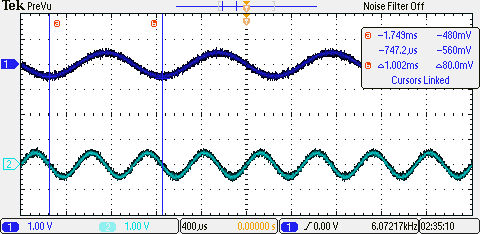
\includegraphics[width=0.65\textwidth]{img/task1.PNG}
    \caption{Blue: 1kHz Green: 2kHz.}
  \end{center}
\end{figure}

\begin{figure}[h]
  \begin{center}
    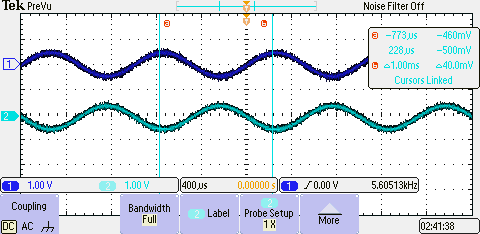
\includegraphics[width=0.65\textwidth]{img/task2.PNG}
    \caption{Blue: 1kHz Green: 7kHz.}
  \end{center}
\end{figure}

\begin{figure}[h]
  \begin{center}
    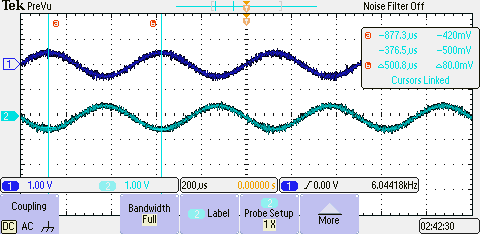
\includegraphics[width=0.65\textwidth]{img/task3.PNG}
    \caption{Blue: 2kHz Green: 6kHz.}
  \end{center}
\end{figure}

%----------------------------------------------------------------------------------------
%	SECTION 4
%----------------------------------------------------------------------------------------

\section{Discussion}

\subsection{Difference Equation}
\subsection{EDMA: Look Up Table}

In part 1 we had issues setting the initial conditions for the difference equation.
We copied the code from the book, but we overlooked a scaling factor that seemed inconsequential.
To fix the problem we ended up using a flag to initialize the variables at the start of the ISR.

In part 2 we had issues initializing the LUT.
We realized that we were typecasting in the wrong order which caused us to have significant roundoff error.
We fixed our error by breaking up our statement into multiple statements.

%----------------------------------------------------------------------------------------
%	SECTION 5
%----------------------------------------------------------------------------------------

\section{Answers questions}

\subsection{Difference Equation}
\subsection{EDMA: Look Up Table}

\begin{enumerate}
  \begin{item}
    Explain what happened mathematically.

  \textbf{Answer:}

  \end{item}

  \begin{item}
    What is aliasing? How do you manage aliasing in DSP applications?

  \textbf{Answer:}
    Aliasing is when the high frequency content of your analog signal appears to be at a lower frequency in discrete time.
    To prevent aliasing in our applications we will filter the input signal with a lowpass filter that has a cutoff frequency of $\frac{f_s}{2}$.
  \end{item}

  \begin{item}
    Change the code in the “ISRs.c” file to implement: talk-through with swap (left channel; right channel). You don’t have to run the project or show the result. Just write down the necessary code.

  \textbf{Answer:}
    \begin{verbatim}
    float temp;

    temp = CodecData.channel[RIGHT];
    CodecData.channel[RIGHT] = CodecData.channel[LEFT];
    CodecData.channel[LEFT] = temp;
    \end{verbatim}
  \end{item}

  \begin{item}
    How are 32-bit floating-point results saved on the 'C6000 processors? Explain briefly the IEEE single-precision floating-point format. When does the 'C6000 use IEEE single-precision floating-point format (i.e give an example of an operation)

  \textbf{Answer:}
    32-bit floating point numbers are stored in IEEE single precision floating point format.
    IEEE format reserves one bit for sign, followed by 8 exponent bits, followed by 23 mantisa bits.
    The exponent is excess 127, and the mantisa is normalized so the leading bit is a one.
    The 'C6000 uses single precision when only floats are invloved i.e. ($1.0F + 1.0F$).
  \end{item}

  \begin{item}
    How does the scheduler work in DSP/BIOS?

  \textbf{Answer:}
    The scheduler periodically interrupts the current thread and determines what the highest priority thread is that is ready to execute.
  \end{item}

  \begin{item}
    What are the different threads present in DSP/BIOS? State the names in descending order of priority and describe in brief the function of each thread.

  \textbf{Answer:}
    Hardware Interrupt, triggered by hardware, used to transfer data or to trigger software interrupts.
    Software Interrupt, used to handle involved processing.
    Periodic Function, similar to software interrupt, but scheduled at regular intervals.
    Tasks, functions that handle the most complex processing.
    Idle Functions, used for system maintenance when there are no pending threads.
  \end{item}

  \begin{item}
    How will you determine the number of clock cycles required to execute your program?

  \textbf{Answer:}
    By changing the state of a logical signal upon entering and leaving my ISR, and monitoring that signal with an osciloscope.
  \end{item}

  \begin{item}
    How does an external processor access the entire memory space of the DSP?

  \textbf{Answer:}
    Using the enhanced direct memory access controller.
  \end{item}

  \begin{item}
    What is the purpose of the board support library?

  \textbf{Answer:}
    To standardize access to DSP hardware.
  \end{item}
\end{enumerate}

%----------------------------------------------------------------------------------------
%	BIBLIOGRAPHY
%----------------------------------------------------------------------------------------

\bibliography{mybib}
\bibliographystyle{plain}

%----------------------------------------------------------------------------------------


\end{document}
